\documentclass[11pt]{article}
\usepackage{fontspec}
\usepackage{lmodern}
\usepackage{amsmath,amsthm,mathtools}
\usepackage{amsfonts,amssymb}
\usepackage{graphicx,overpic}
\usepackage{hyperref}
\usepackage{microtype}
\usepackage{dsfont}
\usepackage{booktabs}
\usepackage[backend=biber,hyperref=true,backref=true]{biblatex}
\usepackage{fullpage}
\usepackage{float}
\usepackage{subfig}
\bibliography{Biblio}

\graphicspath{{./figures/}}

\newcommand{\sgn}{\operatorname{sgn}}
\newcommand{\conv}{\operatorname{conv}}
\newcommand{\vect}{\operatorname{vect}}
\DeclareMathOperator*{\argmin}{arg\,min}
\DeclareMathOperator*{\argmax}{arg\,max}
\newcommand*\diff{\mathop{}\!\mathrm{d}}
\newcommand{\Var}{\mathrm{Var}}
\newcommand*\ri{\mathop{}\!\mathrm{ri}}
\newcommand*\aff{\mathop{}\!\mathrm{aff}}
\newcommand*\dom{\mathop{}\!\mathrm{dom}}
\newcommand*\epi{\mathop{}\!\mathrm{epi}}
\newcommand*\diag{\mathop{}\!\mathrm{diag}}
\newcommand*\cov{\mathop{}\!\mathrm{cov}}
\newcommand*\var{\mathop{}\!\mathrm{var}}
\newcommand*\corr{\mathop{}\!\mathrm{corr}}


\begin{document}
\date{9 December 2016}
\author{Guillaume Ausset}
\title{Blind source separation using ICA}
\maketitle

\emph{All my code, report, poster and any other material will be tracked with \text{Git}. The repository is at \url{https://gitlab.com/aussetg/pgm-ica} but is private before the presentation, if you want access just ask me at \href{mailto:guillaume@ausset.me}{\nolinkurl{guillaume@ausset.me} } and I will gladly add you.}

\section{Introduction of the Problem}

It is quite common when measuring several signals at once to be unable a priori to isolate the different source signals and only be able to observe a mixture of those sources. When recording sound the signal recorded will be a mixture of different ambient sounds and the sound of interest, when acquiring EEGs eye movement and muscle twitching will be mixed with the main signal. One finds themselves before a problem of the form:

\begin{align*}
	\mathbf{x} = A \mathbf{s}
\end{align*} 

Where $\mathbf{x}$ are our observations, $\mathbf{s}$ our unknown signal of origin and $A$ the mixing matrix.
The problem seems intractable but we will see that only making the hypothesis that the $s_i$ are independent (and eventually some more simplifying hypothesis) make it tractable.

The problem then becomes:
\begin{itemize}
	\item Find a measure of independence, or contrast function.
	\item Maximize that measure with respect to $A$.
\end{itemize}

Therefore for each measure of independence chosen we find a new method to solve ICA.

\section{Methods that will be implemented}

\subsection{Fast-ICA}

The performance of a given ICA method will depend on the quality of the measure of independence and this measure will also impact the computational complexity of the algorithm. We will therefore try to compare different methods.

The canonical method because of its extreme simplicity and speed is Fast-ICA \cite{Hyvarinen2000}, which chose as a contrast function the negentropy:
\begin{align*}
	J(y) = H(y_\text{gauss}) - H(y)
\end{align*}

with $H(y)$ the differential entropy, $y_\text{gauss}$ a Gaussian variable with the same variance as $y$.

And they give as an approximation if we consider that $y$ is standardized:

\begin{align*}
	J(y) \simeq \left[ \mathbb{E} \left[ G(y) \right] - \mathbb{E} \left[ G(\nu) \right] \right]^2
\end{align*}

with $\nu \sim \mathcal{N} (0,1)$ and $G$ a non-linear and non-quadratic function. This formulation enables the authors to give a very efficient algorithm to maximize $J$ that I have implemented in Julia. See appendix for figures illustrating the different steps of FastICA on completely artificial data.

\subsection{Kernel-ICA}

The idea of \cite{Bach2002} is to optimize the contrast function:

\begin{align*}
	\rho_{\mathcal{F}} = \max_{f_1, f_2 \in \mathcal{F}} \frac{\cov(f_1 (x_1), f_2(x_2))}{(\var f_1(x_1))^{1/2} (\var f_2(x_2))^{1/2}}
\end{align*}

Or more precisely a penalized version of that contrast function. Direct computation of this function seems intractable especially if $\mathcal{F}$ is big enough, the authors therefore chose $\mathcal{F}$ as a reproducing kernel Hilbert space in order to exploit the kernel "trick" so as to transport the problem from the space $\mathcal{F}$ to $\mathcal{X}$ the feature space:

\begin{align*}
	\corr(f_1(x_1), f_2(x_2)) = \corr \left( \langle \Phi (x_1), f_1 \rangle, \langle \Phi (x_2), f_2 \rangle \right)
\end{align*}

where $\Phi$ is the map associated to the kernel of the space and the problem is then a form of Kernel CCA which is tractable.

Kernel-ICA will be implemented in Julia and contrasted with Fast-ICA.

\section{Possible extension}

While I have not yet entirely read the papers and will concentrate on implementing Kernel-ICA first, I hope to be able to compare the two previous methods to a variational approach of ICA as in \cite{Lawrence2000, Winther2007, Choudrey2002}.

\section{Results}

We generate points uniformly on $[0,10]^2$ and then mix them with:

\begin{align*}
	\begin{pmatrix}
		1 & 2 \\ 
		21 & 20
	\end{pmatrix}	
\end{align*}

And then use FastICA to retrieve the original components.

Note that it is completely normal that the retrieved components have different amplitudes, it's impossible to retrieve the amplitude and the sign. I, however, forgot to add back the mean.

\begin{figure}[H]
  \centering
  \subfloat[$s$ original]{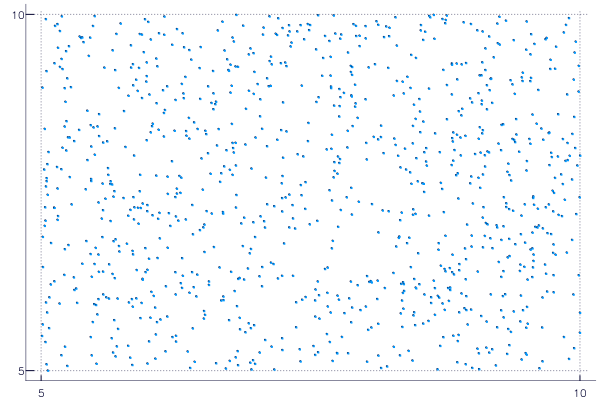
\includegraphics[width=0.45\textwidth]{s_orig.png}}
  \hfill
  \subfloat[$x = A s$]{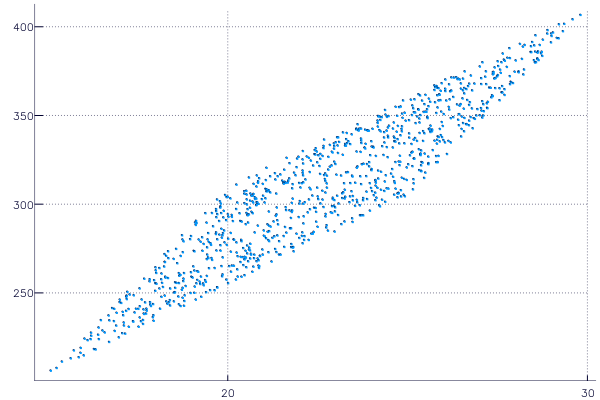
\includegraphics[width=0.45\textwidth]{x.png}}
  \caption{Independent components and their mixture}
\end{figure}

\begin{figure}[H]
  \centering
  \subfloat[$x$ centered]{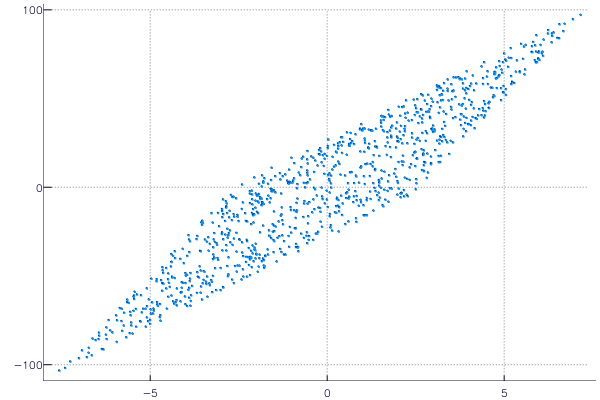
\includegraphics[width=0.45\textwidth]{x_c.png}}
  \hfill
  \subfloat[$x$ whitened]{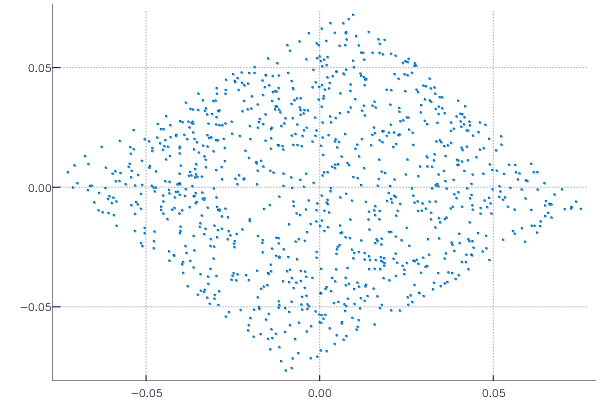
\includegraphics[width=0.45\textwidth]{x_w.png}}
  \caption{Preprocessing}
\end{figure}

\begin{figure}[H]
 	\centering
	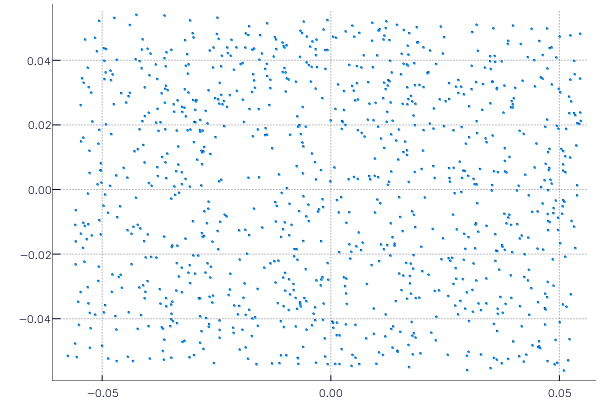
\includegraphics[width=0.5\textwidth]{s_retrieved.png}
 	\caption{Final retrieved $s$}
\end{figure}

\printbibliography

\end{document}
